\documentclass[a4paper]{article}
\usepackage[utf8]{inputenc}
\usepackage{polyglossia} % Language support for XeLaTeX/LuaLaTeX
\setmainlanguage{latvian}
\setotherlanguage{english}
\usepackage[margin=2cm]{geometry}
\usepackage{graphicx}
\usepackage{caption}
\usepackage{amsmath}
%\usepackage{array}
%\usepackage{multirow}
%\usepackage{float}
%\usepackage{hyperref}
%\usepackage{listings}
\usepackage[
  backend=biber,
  style=phys, % or choose a different style (e.g., numeric, authoryear)
]{biblatex}
\addbibresource{references.bib}

\title{Viskozitātes noteikšana šķidrumos un gāzēs}
\author{Elīna Neilande}
\date{November 2024}

\begin{document}

\maketitle

\section{Ievads}

Šķidrumiem un gāzēm piemīt viskozitāte, kad šķidruma vai gāzes slāņi nav relatīvā miera stāvoklī viens pret otru. Slāņi iedarbojas viens uz otru. Starp slāņiem parādās miejiedarbības spēks -- berzes spēks. Šo berzi sauc par iekšējo berzi. Iekšējā berze (viskozitāte) šķidrumos un gāzēs pastāv tādēļ, ka notiek molekulu pāreja starp slāņiem, kas pārvietojas ar dažādiem ātrumiem. Molekulas, pārejot no ātrākiem slāņiem uz lēnākiem slāņiem, paātrina lēnākos slāņus un tie sāk pārvietoties ātrāk. Ja molekulas no lēnākiem slāņiem nonāk ātrākos slāņos, bremzē tos, skat. att.~\ref{fig:vis}.

\begin{figure}
    \centering
    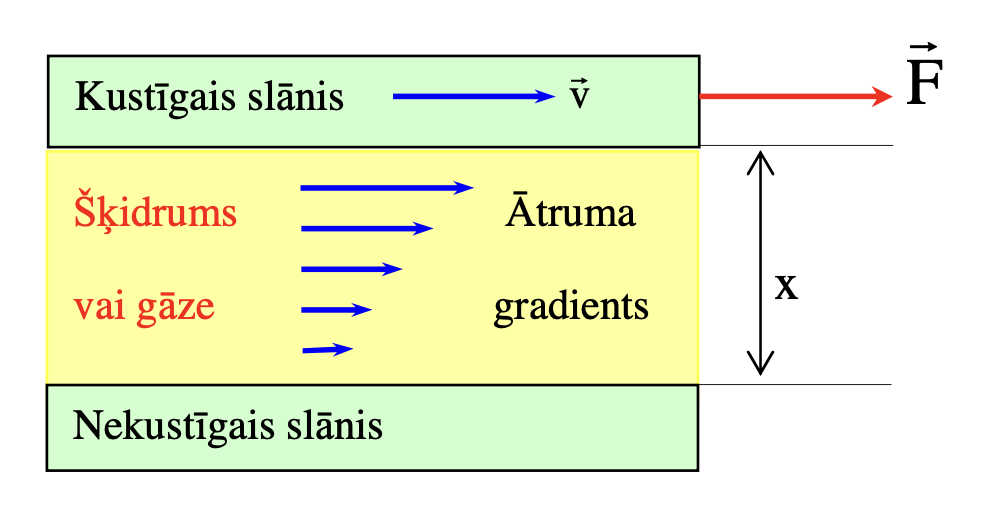
\includegraphics[width=0.75\textwidth]{1att.png}
    \caption{Viskozitāte šķidrumos un gāzēs.}
    \label{fig:vis}
\end{figure}

Vielā parasti nav tādu norobežotu slāņu, kuros ir viens noteikts ātrums, bet ātrums slānī nepārtraukti mainās. Ātruma raksturošanai ievieš ātruma gradientu 
\begin{equation}
    \text{grad}(v) = \frac{dv}{dx} .
\end{equation}

Ja attālums starp diviem slāņiem ir \( x \) un otrā slāņa ātrums attiecībā pret pirmo slāni ir \( v \), tad, pieņemot, ka ātrums mainās lineāri atkarībā no attāluma, ātruma gradients ir 
\begin{equation*}
    \frac{dv}{dx} = \frac{v}{x} .
\end{equation*}

Slāņu iekšējās berzes spēks \( F \) ir atkarīgs no slāņu, starp kuriem pastāv berze, saskares virsmas laukuma \( S \) un ātruma gradienta:
\begin{equation} \label{eq:2}
    F = \eta \cdot S \cdot \frac{dv}{dx} ,
\end{equation}
kur \( \eta \) ir proporcionalitātes koeficients, ko sauc par iekšējās berzes jeb viskozitātes koeficientu. Sakarību \ref{eq:2} sauc par Furjē formulu.
\pagebreak
\section{Laminārā un turbulenta plūsma}

\begin{figure}[h]
    \centering
    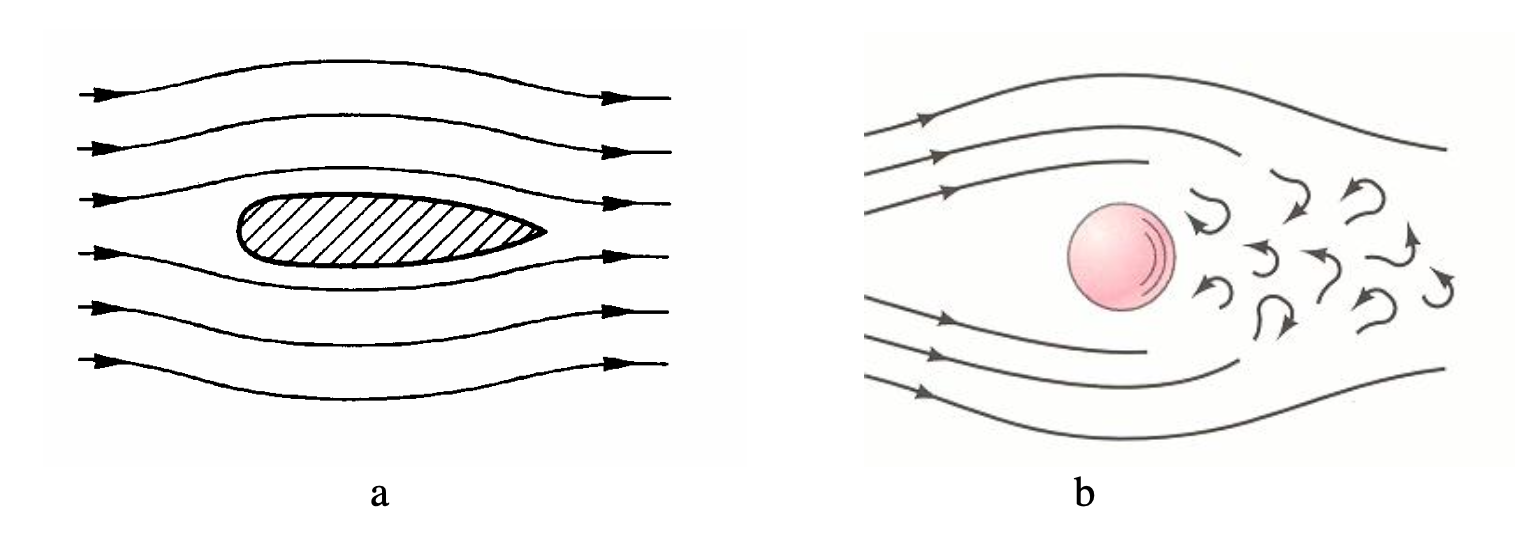
\includegraphics[width=0.75\textwidth]{2att.png}
    \caption{Lamināra (a) un turbulenta (b) plūsma.}
\end{figure}

Pētot lamināru plūsmu caur kapilāru Hāgens 1839.g. \cite{Hagen1839} un Puazeils (\textit{Poiseuille}) 1840.g. \cite{Sutera2003} eksperimentāli atklāja, ka laminārā šķidruma vai gāzes plūsmā laika vienībā caur kapilāra šķērsgriezuma laukumu izplūdušā šķidruma vai gāzes tilpumu \( V_0 = \frac{V}{t} \) nosaka sakarība:
\begin{equation}
    V_0 = \frac{\pi \cdot \Delta p \cdot R^4}{8 \cdot \eta \cdot L},
\end{equation}
kur \( R \) ir kapilāra rādiuss, \( L \) ir kapilāra garums, \( \Delta p \) ir spiediena starpība starp kapilāra galiem, un \( \eta \) ir viskozitātes koeficients: 
\begin{equation} \label{eq:4}
    \eta = \frac{\pi \cdot \Delta p \cdot R^4 \cdot t}{8 \cdot L \cdot V} .
\end{equation}

Lamināru šķidrumu vai gāzes plūsmu caurulēs raksturo Reinoldsa skaitlis:
\begin{equation}\label{eq:5}
    R_e =2,718 \frac{\rho \cdot v \cdot d}{\eta},
\end{equation}
kur \( \rho \) -- šķidruma vai gāzes blīvums, \( d \) -- caurules diametrs, \( v \) -- šķidruma vai gāzes plūsmas ātrums, \( \eta \) -- šķidruma vai gāzes viskozitātes koeficients.

Lai plūsma būtu lamināra, reinoldsa skaitlim jābūt mazākam par 2000 \cite{rhodes2008}. Laika vienībā caur kapilāru izplūdušā šķidruma (gāzes) tilpums \( V_0 = v \cdot S \) un kapilāra šķērsgriezuma laukums \( S = \frac{\pi \cdot d^2}{4} \), no šīm abām izteiksmēm izsaka plūsmas ātrumu:
\begin{equation}
    v = \frac{V_0}{S} = \frac{4 \cdot V_0}{\pi \cdot d^2}.
\end{equation}

No izteiksmēm \ref{eq:4} un \ref{eq:5} iegūst:
\begin{equation}
    R_e =2,718 \frac{4 \cdot \rho \cdot V_0}{\pi \cdot d \cdot \eta}.
\end{equation}
\pagebreak
\section{Stoksa likums}

Kustoties šķidrumā cietam ķermenim, tas viskozitātes dēļ aizrauj līdzi tam pieguļošos šķidruma slāņus, tāpēc šķidrums izrāda pretestību ķermeņa kustībai. Pretestības spēks ir atkarīgs no vides, ķermeņa kustības ātruma, tā izmēriem un formas. Mazu kustības ātrumu gadījumā pretestības spēks ir proporcionāls ķermeņa kustības ātrumam. Stokss konstatēja, ka sfēriskas formas ķermeņiem, kas kustas ar nelielu ātrumu, šķidruma pretestības spēks \( \vec{F} \) ir proporcionāls ķermeņa kustības ātrumam \( v \) un lodes rādiusam \( r \):
\begin{equation}\label{eq:7}
    F = 6\pi\eta r v,
\end{equation}
kur \( \eta \) -- viskozitātes koeficients.
Sakarību \ref{eq:7} sauc par Stoksa likumu \cite{Stokes}. 

Uz lodi, kuras masa \( m \) un rādiuss \( r \), kas krīt ar ātrumu \( v \) šķidrumā, kura viskozitātes koeficients ir \( \eta \), darbojas 3 spēki (skat. \ref{fig:forces} att.). Šie spēki ar laiku līdzsvarojas.

\begin{figure}[h]
    \centering
    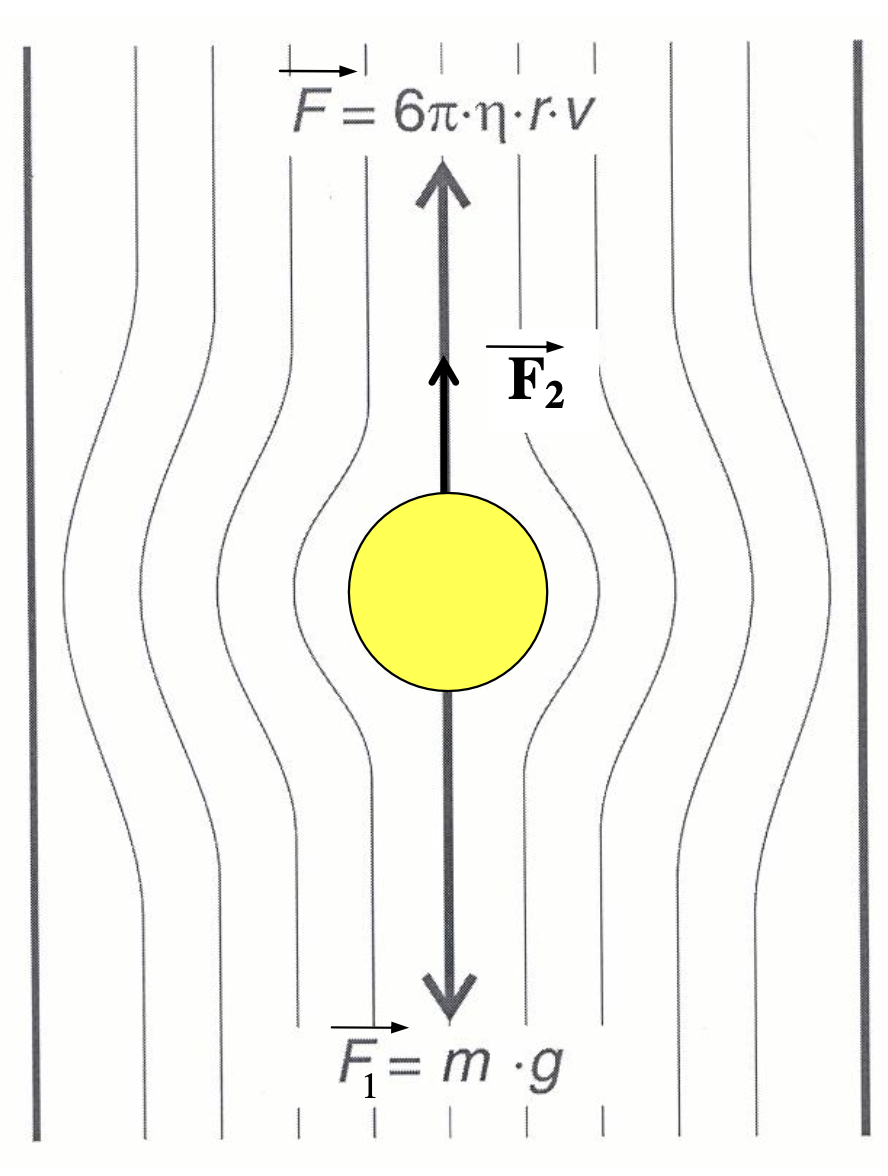
\includegraphics[width=0.5\textwidth]{3att.png}
    \caption{Ķermeņa krišana šķidrumā vai gāzē.}
    \label{fig:forces}
\end{figure}

Lodes smaguma spēks ir
\begin{equation}\label{eq:F1}
    F_1 = mg = \frac{4}{3}\pi r^3 \rho g 
\end{equation}
un uz lodi darbojas Arhimēda spēks:
\begin{equation}\label{eq:F2}
    F_2 = \frac{4}{3}\pi r^3 \rho_0 g ,
\end{equation}
kur \( r \) -- lodes rādiuss, \(m\) -- lodes masa, \(g\) -- brīvās krišanas paātrinājums, \(\rho\) -- lodes blīvums un \(\rho_0\) -- šķidruma blīvums.

Ievietojot izteiksmē \ref{eq:7} izteiksmes \ref{eq:F1} un \ref{eq:F2}, iegūst
\begin{equation*}
    \frac{4}{3}\pi r^3 \rho g = 6\pi \eta r v + \frac{4}{3}\pi r^3 \rho_0 g,
\end{equation*}
no kurienes seko:
\begin{equation}\label{eq:eta}
    \eta = \frac{2 \cdot r^2 \cdot g \cdot (\rho - \rho_0}{9 \cdot v} = \frac{1}{18}\cdot g \cdot (\rho-\rho_0)\cdot \frac{d^2\cdot t}{s},
\end{equation}
kur \(d\) -- lodes diametrs un \(s\) -- lodes veiktais ceļš laikā \(t\).

Izteiksme \ref{eq:eta} ir izmantojama tikai tad, ja vide, kurā kustās lode, ir neierobežota (bez sienām) un lode kustības laikā nedeformējas. Praksē šķidrums ir iepildīts cilindriskas formas traukā, kura diametrs ir \(D\). Lode krīt pa cilindra asi. Vienādojumu nepieciešams koriģēt:
\begin{equation}
    \eta = \frac{1}{18}\cdot g \cdot (\rho-\rho_0) \cdot \frac{d^2 \cdot t}{s \cdot (1 + 2,4 \cdot \frac{d}{D})}
\end{equation}

\printbibliography

\pagebreak

\section{Pielikums}

\begin{table}[h]
    \centering
    \begin{tabular}{|c|c|c|c|}
        \hline
        \textbf{Temperatūra ($^\circ$C)} & \textbf{Ūdens (Pa$\cdot$s)} & \textbf{Glicerīns (Pa$\cdot$s)} & \textbf{Etanols (Pa$\cdot$s)} \\
        \hline
        10 & $1.30 \times 10^{-3}$ & 3.950 & $1.47 \times 10^{-3}$ \\
        20 & $1.00 \times 10^{-3}$ & 1.480 & $1.20 \times 10^{-3}$ \\
        30 & $0.80 \times 10^{-3}$ & 0.600 & $1.00 \times 10^{-3}$ \\
        40 & $0.65 \times 10^{-3}$ & 0.330 & $0.83 \times 10^{-3}$ \\
        50 & $0.55 \times 10^{-3}$ & 0.180 & $0.70 \times 10^{-3}$ \\
        60 & $0.47 \times 10^{-3}$ & 0.102 & $0.59 \times 10^{-3}$ \\
        70 &  & 0.059 & $0.50 \times 10^{-3}$ \\
        80 &  & 0.035 &  \\
        \hline
    \end{tabular}
    \caption{Šķidrumu viskozitātes koeficienta atkarība no temperatūras (\( \eta, Pa \cdot s\))}
    \label{tab:viscosity}
\end{table}

\end{document}